
\section{Ecuaciones de movimiento de cuerpo rígido} \label{sec:ecuacionesRigid}
Se hará referencia a la figura \ref{fig:FBD2D} para explicar las variables en juego en el modelo 3D debido a la dificultad inherente de mostrar las 16 variables de estado en un dibujo del modelo 3D.

\begin{figure}[htb!]
	\centering
	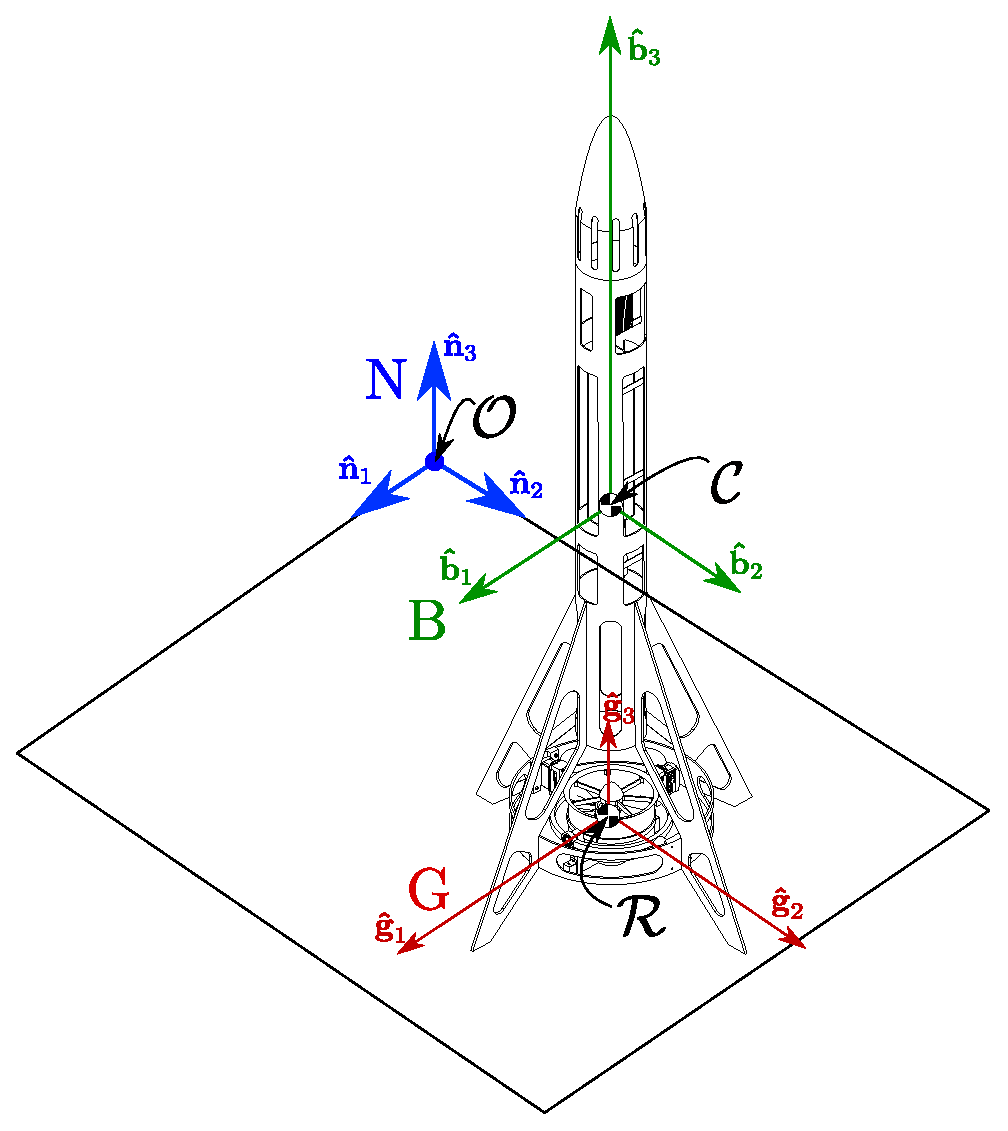
\includegraphics[width=0.52\textwidth]{fig/marcosDiagrama.eps}
	\caption{Marcos de referencia tomados para el análisis de cuerpo rígido. Por simplicidad se toman los centros de masa del cardán y del rotor como coincidentes en el punto $\ogn{R}$.}
\end{figure}

\subsection{Notación}

La notación es la del libro \textit{Rigid Body Dynamics of Mechanisms, Theoretical Basics} \cite{hahn2013rigid}. Se requiere un tratamiento algebraico explicito de los marcos de referencia y representación debido al caso especial de un \textit{gimballed rotor}. Este tratamiento facilita la programación de la simulación y subsecuentemente el control, el cual se volvería ambiguo y complejo con un tratamiento más común o simplificado.

\begin{description}
	\item[{\(\avec{r}_{\ogn{CO}}=[x,y,z]\)}] : Posici\'on absoluta del centro de masa del veh\'iculo leasé ``posición de $\ogn{C}$ respecto $\ogn{O}$'')
	\item[{\(\avec{r}_{\ogn{RC}}\)}] : Posición del centro de masa del cardán respecto al centro de masa del vehículo
	\item[{\( \avec{\eta}=[\phi,\theta,\psi] \)}] : Ángulos de actitud del vehículo (Ángulos Euler)
	\item[\( \avec{\omega}_r^{\frm{G}} \)] : Velocidad angular del rotor del EDF representado en el marco $\frm{G}$ (dirección constante)
	\item[\( \avec{\omega}_\frm{BN}^\frm{B} \)] : Velocidad angular de $\frm{B}$ respecto a $\frm{N}$, representado en el marco $\frm{B}$.
	\item[\(  \alpha, \beta \)] : Ángulo de actuación de vectorización del EDF o ángulo de actitud del marco $\frm{G}$
	\item[{\( \delta   \)}] :  Ángulo de actuación de los dos flaps anti-roll
	\item[{\( m  \)}] :  Masa del vehículo sin rotor
	\item[{\( m_r  \)}] :  Masa del rotor
	\item[{\( \avec{g}  \)}] :  Aceleración de la gravedad
	\item[{\( \avec{F}^\frm{B} \)}] : Empuje del EDF representado en el marco $\frm{B}$ 
	\item[{\( \transform{NB}  \)}] :  Matriz de transformación de cosenos directores de un marco $\frm{B}$ a el marco $\frm{N}$
\end{description}

\textbf{Caracterización del EDF}
\begin{description}
	\item[{\( \tau_c  \)}] :  Torque efectivo de control del EDF
%	\item[{\( i  \)}] :  Corriente entregada al motor
	\item[{\( K_T  \)}] :  Constante de empuje del EDF
	\item[{\( K_Q  \)}] :  Coeficiente de torque viscoso de fricción
	\item[{\( Q  \)}] :  Torque viscoso de fricción
	\item[{\( \tau_r \)}] : Torque de reacción por el swirl de salida
\end{description}

\textbf{Caracterización del mecanismo anti-roll:}
\begin{description}
	\item[{\( K_{F_L}  \)}] : Coeficiente de lift de los flaps anti-roll
	\item[{\( K_{F_D}  \)}] : Coeficiente de drag de los flaps anti-roll
	\item[{\( F_L \)}] : Lift de los flaps anti-roll
	\item[{\( F_D \)}] : Drag de los flaps anti-roll
\end{description}

\textbf{Matriz de inercia:}
\begin{description}
	\item[{\(  \inertia{C}{B}  \)}] : Vehículo sin rotor respecto a $\ogn{C}$ representado en $\frm{B}$
	\item[{\(  \inertiarotor{R}{G}  \)}] : Rotor respecto a $\ogn{R}$ representado en $\frm{G}$
	\item[{\(  \inertia{\!\mathrm{g}R}{G}  \)}] : Cardán y motor sin rotor respecto a $\ogn{R}$ representado en $\frm{G}$
\end{description}



\subsection{Notación del álgebra a utilizar}

El producto escalar se define como $\bigcdot$ para diferenciarlo de simple multiplicación vectorial ($\cdot$). $\skw{\omega}$ es la matriz skew del vector que reemplaza el producto vectorial ya que $\skw{r}\cdot v = r \times v$
\[
\skw{\omega}_{L R}^{L}=\left(\begin{array}{ccc}
0 & -\omega_{z L R}^{L}, & \omega_{y L R}^{L} \\
\omega_{z L R}^{L} & 0 &-\omega_{x L R}^{L} \\
-\omega_{y L R}^{L} &  \omega_{x L R}^{L} & 0
\end{array}\right)
\]

Se dice que $J_\ogn{C}^\frm{B}$ es la matriz de inercia respecto el punto $\ogn{C}$, representado en el marco $\frm{B}$: es decir, las componentes de la matriz de inercia están en la base de $\frm{B}$. Esto se puede escribir así:
\begin{IEEEeqnarray*}{c}
J_\ogn{C}^\frm{B} = J_{b1} \bvec{b}_1 + J_{b2} \bvec{b}_2 + J_{b3} \bvec{b}_3
\end{IEEEeqnarray*}

La derivada del término anterior respecto un marco $N$ quedaría escrito
$${}^\frm{N}\dot{J}_{\ogn{C}}^\frm{B} =\left.^\frm{N} \frac{\di J_\ogn{C}^\frm{B}}{\di t}  \right. = \transform{NB} \cdot \left.^\frm{B} \frac{\di J_\ogn{C}^\frm{B}}{\di t}  \right. $$


Se pueden demostrar las siguientes ecuaciones
\begin{IEEEeqnarray}{C}
\dottransform{RL} =\transform{RL}\cdot \skw{\omega}^\frm{L}_\frm{LR} =
\skw{\omega}^\frm{R}_\frm{LR}\cdot\transform{LR} = -\skw{\omega}^\frm{L}_\frm{LR}\cdot\transform{RL} \\
\transform{BN} = (\transform{NB})\tp =  (\transform{NB})^{-1} \quad \Rightarrow \quad \transform{NB} \cdot \transform{BN} = \eye
\end{IEEEeqnarray}

donde $\omega_{\frm{LR}}^{\frm{L}}$ es la velocidad angular vectorial del marco $\frm{L}$ con respecto a $\frm{R}$ representado en $\frm{L}$, $\transform{RL}$ es la matriz de cosenos directores que transforma una vector de una base ortogonal $\frm{L}$ a otra base ortogonal $\frm{R}$, y $\dottransform{RL}$ es la derivada de la matriz $\transform{RL}$ respecto $\frm{R}$.


\subsection{Variables de estado}
Se tendrán las variables de estado de posición y velocidad donde $z$ positivo es alejándose de la tierra.
\[
\avec{r}_\ogn{CO}^\frm{N} = 
\begin{bmatrix}
x & y & z 
\end{bmatrix}, \qquad
\dot{\avec{r}}_\ogn{CO}^\frm{N} = 
\begin{bmatrix}
\dot{x} & \dot{y} & \dot{z}
\end{bmatrix} 
\]

El movimiento cuerpo rígido será descrito por 3 ángulos de Euler (Cardán o Bryant en algunas bibliografías) $\phi, \theta$ y $\psi$ (roll, pitch, yaw respectivamente).
\begin{IEEEeqnarray}{C}
\avec{\eta} = \begin{bmatrix}
\phi  &  \theta &  \psi
\end{bmatrix}
\end{IEEEeqnarray}

\begin{figure}[ht!]
	\centering
	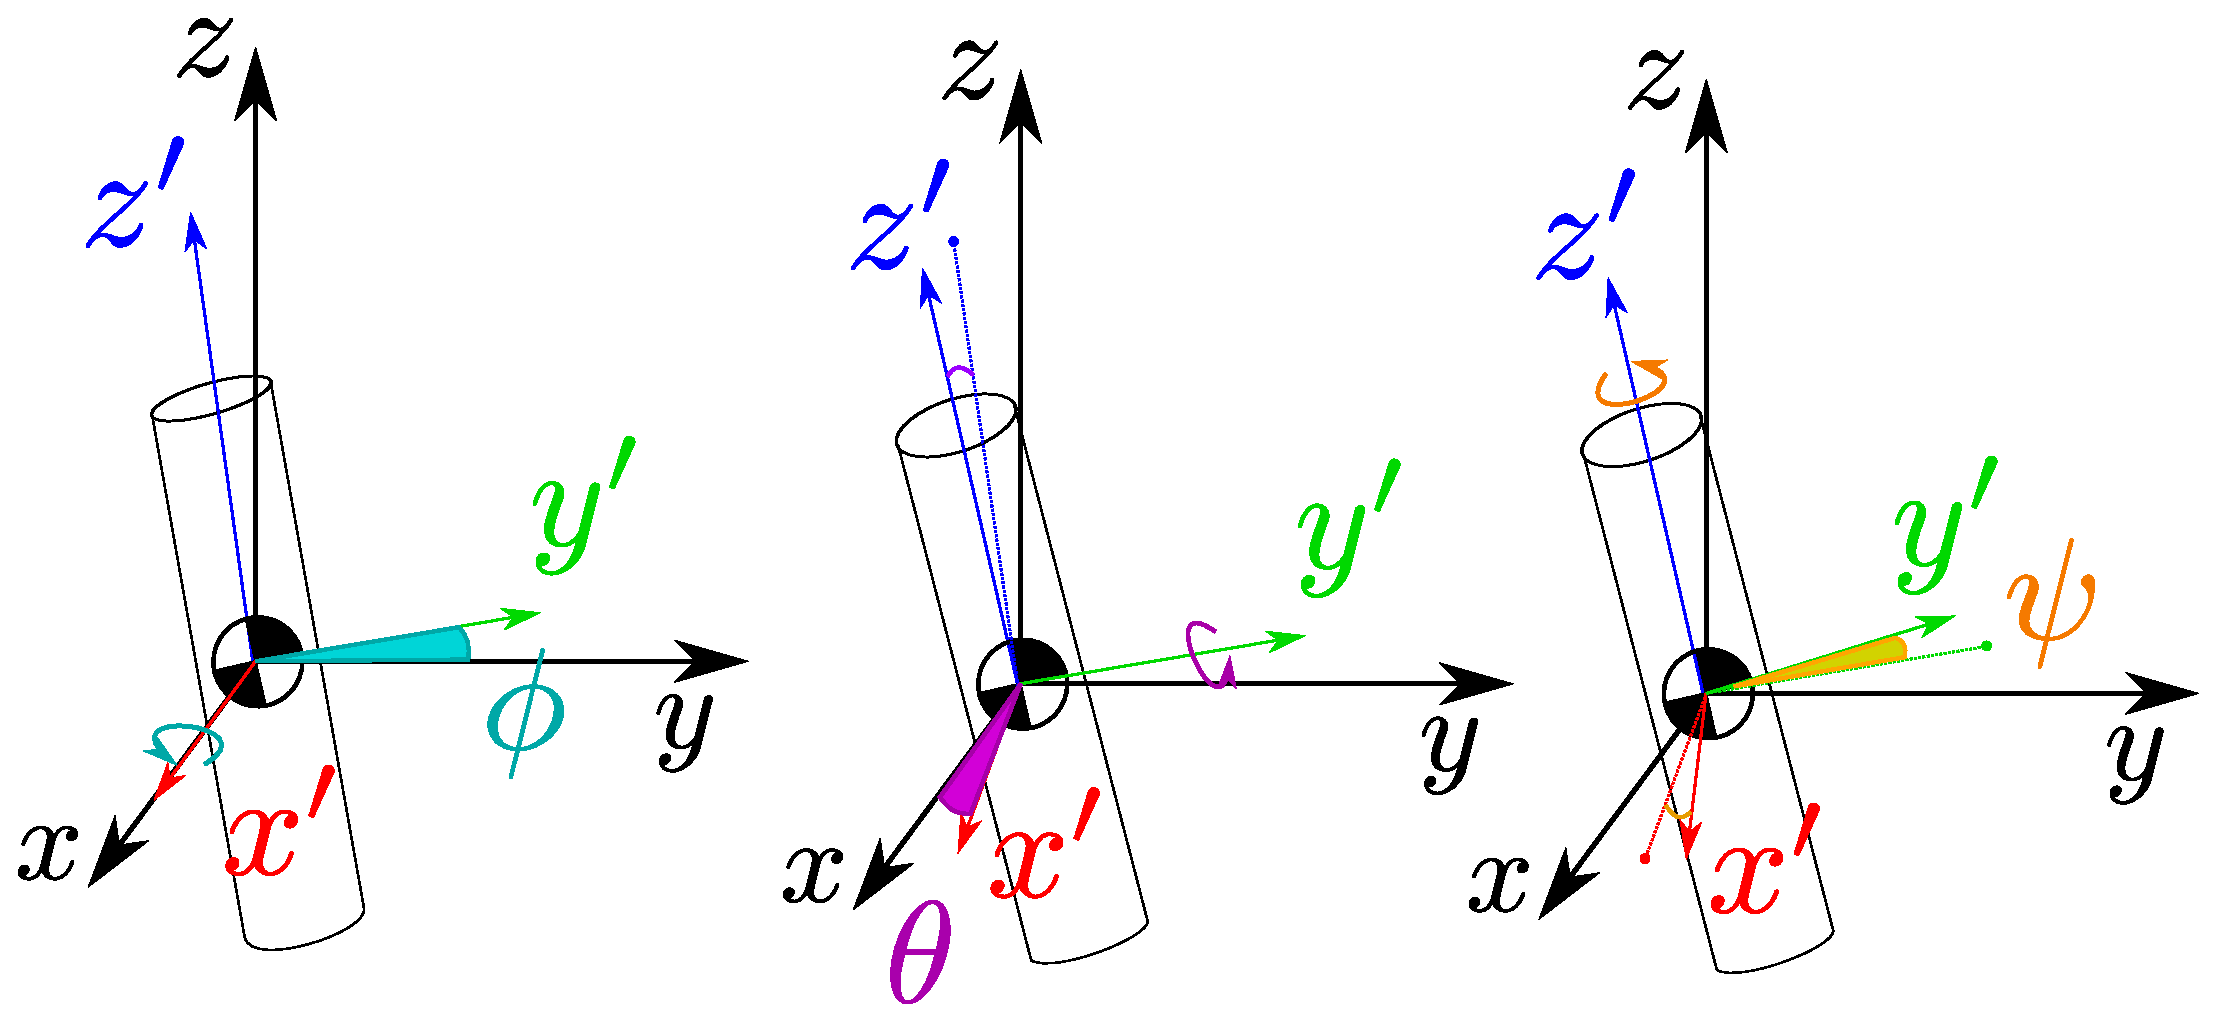
\includegraphics[width=0.8\textwidth]{fig/cuerpolibreGlobal_v2.eps}
	\caption{Diagrama mostrando las rotaciones de ángulo de euler en el orden que son efectuadas para describir el sistema. $\phi$ representa el pitch, $\theta$ el yaw y $\psi$ el roll. Se muestran las últimas posiciones de los ejes rotados con una linea punteada.}
\end{figure}


Los ángulos de la vectorización de la tobera serán $\alpha$ y $\beta$. $\delta$ corresponde a los actuadores que contrarrestan el roll del vehículo mediante dos flaps. Los ángulos $\alpha$ y $\beta$ describen la dirección en la que está apuntando la tobera (equivalente a la orientación $\frm{G}$) respecto la dirección del vehículo (marco $\frm{B}$). $\omega_r=\omega_r^\frm{G}$ es la velocidad angular del rotor.

Se escriben las variables de estado y el vector input, donde $F$ es la fuerza que hace la tobera sobre el vehículo (la cual depende de la velocidad del vehículo)\footnote{En el código $\phi$, $\theta$ y $\psi$ aparecen como \texttt{q,r,s}}
\begin{equation} \label{eq:ssVariables3D}
	\Cx = \left[
	\begin{array}{cccccccc}
		\avec{r}_\ogn{CO}^\frm{N} & \avec{\eta} &\dot{\avec{r}}_\ogn{CO}^\frm{N} &  \avec{\omega}_\frm{BN}^\frm{B} & \omega_r & \alpha & \beta & \delta
	\end{array}\right] \tp
\end{equation}
\begin{equation}\label{eq:ssInputs3D}
	\Cu = \begin{bmatrix}
		\tau_c & \dot{\alpha} & \dot{\beta} & \dot{\delta}
	\end{bmatrix} \tp
\end{equation}
En la próxima sección se buscará obtener el vector de variables de estado derivado en el tiempo $\dot{\Cx}$.

\subsection{Ecuaciones diferenciales} \label{subsec:modeloMatematico}

\def\scos{\operatorname{c}}
\def\ssin{\operatorname{s}}
Definimos la transformación de los ángulos euler con una matriz de transformación $\transform{BN}$ donde $\scos$ y $\ssin$ son las funciones coseno y seno, respectivamente.

\begin{equation} \label{eq:matrizTransfoVehiculo}
	\transform{BN} = \begin{bmatrix}
	\scos \theta \cdot \scos \psi & \scos \theta \cdot \ssin \psi & - \ssin \theta \\
	\ssin \phi \cdot \ssin \theta \cdot \scos \psi - \scos \phi \cdot \ssin \psi & \ssin\phi \cdot \ssin\theta \cdot \ssin\psi + \scos\phi\cdot\scos\psi & \ssin\phi \cdot \scos\theta \\
	\scos\phi \cdot \ssin\theta \cdot \scos\psi + \ssin\phi \cdot \ssin\psi\quad & \scos\phi \cdot \ssin\theta \cdot \ssin\psi - \ssin\phi \cdot \scos\psi \quad& \scos\phi \cdot \scos\theta
	\end{bmatrix}
\end{equation}
La transformación nos servirá para poder pasar de la dinámica que está definida en el marco del vehículo $\frm{B}$ al marco $\frm{N}$ donde se tienen las variables de estado que se desean controlar.

Podemos obtener la velocidad en el marco del cuerpo
\begin{IEEEeqnarray}{rCl}
	\dot{\avec{r}}_\ogn{CO}^\frm{B} &= &\transform{BN} \cdot \dot{\avec{r}}_\ogn{CO}^\frm{N} 
\end{IEEEeqnarray}

La obtención de la velocidad angular del cuerpo se complica por el hecho que la razón de cambio de los ángulos de Euler no son vectores cartesianos, si no más bien parámetros que describen la orientación del cuerpo rígido en el espacio.\footnote{ Como bien sabemos la matriz de transformación $\tform$ solo es aplicable para transformar vectores cartesianos de una base ortogonal a otra. Los parámetros $\avec{\eta}$ conforman un vector de configuración, no un vector cartesiano!} Para relacionar la velocidad angular con $\avec{\eta}$ es necesario utilizar la matriz de actitud cinemática $\attitude(\avec{\eta})$.

\begin{IEEEeqnarray}{c}
	\attitude(\avec{\eta}) = \left[\begin{array}{ccc}
	1 & \sin (\phi) \tan (\theta) & \cos (\phi) \tan (\theta) \\
	0 & \cos (\phi) & -\sin (\phi) \\
	0 & \sin (\phi) \sec (\theta) & \cos (\phi) \sec (\theta)
	\end{array}\right]
\end{IEEEeqnarray}

La matriz de actitud cinemática se usa para transformar 
\begin{IEEEeqnarray}{rCl}
	 \dot{\avec{\eta}}& = & \attitude(\avec{\eta}) \cdot  \avec{\omega}_\frm{BN}^\frm{N} \\
	\avec{\omega}_\frm{BN}^\frm{B} & = &\transform{BN}\cdot \avec{\omega}_\frm{BN}^\frm{N}
\end{IEEEeqnarray}
e inversamente
\begin{IEEEeqnarray}{rCl}
	\avec{\omega}_\frm{BN}^\frm{N} & = &\attitude^{-1}(\avec{\eta})\cdot \dot{\avec{\eta}} \\
\end{IEEEeqnarray}


La fuerza que impulsa al vehículo en el marco del cuerpo se obtiene transformando del marco del cardán donde se conocen los componentes, al marco cuerpo. La matriz es calculada reemplazando $\phi\equiv\alpha$, $\theta\equiv\beta$, y $\psi = 0$.
\begin{equation}
	\avec{F}^\frm{B} = \transform{BG} \cdot \avec{F}^\frm{G} 
\end{equation}

La aceleración del centro de masa del vehículo medido en el marco del cuerpo $\frm{B}$ es igualada a la fuerza
\begin{equation}
	{}^\frm{B}\frac{\di }{\di t}\left( \dot{\avec{r}}_\ogn{CO}^\frm{B} \right) = \frac{1}{m+m_r} \cdot \avec{F}^\frm{B}
\end{equation}
luego obtenemos la aceleración en coordenadas globales
\begin{equation}
	\ddot{\avec{r}}_\ogn{CO}^\frm{N} =
	\transform{NB}\cdot {}^\frm{B}\frac{\di }{\di t}\left( \dot{\avec{r}}_\ogn{CO}^\frm{B} \right)- \avec{g}^\frm{N}
\end{equation}

Los momentos actuantes externos en el marco del vehículo respecto su centro de gravedad $\ogn{C}$ están en función del diseño de los flaps anti roll \cite{romarowski2020edf}.

\begin{equation}
	\avec{M}^\frm{B}_\ogn{C} = \skw{\avec{r}}_\ogn{RC}^\frm{B}\cdot \avec{F}^\frm{B} + \transform{BG} \cdot 
	\begin{bmatrix}
		0 \\
		0 \\
		\omega_r^2 K_{F_L}d_T\delta+\tau_r
	\end{bmatrix}  
\end{equation}
%
La aceleración angular en el marco $\frm{B}$ sale del desarrollo de la sección \ref{ssec:ecuacionangular}
\begin{equation}
{}^\frm{B}\frac{\di }{\di t} \left(\avec{\omega}_\frm{BN}^\frm{B} \right) =  \left(\inertia{C}{B}\right)^{-1} \cdot \left( - \skw{\avec{\omega}}_\frm{BN}^\frm{B} \cdot \inertia{C}{B}\cdot \avec{\omega}_{\frm{BN}}^{\frm{B}} - 
\transform{{BG}} \cdot\skw{\avec{\omega}}_\frm{GB}^\frm{G} \cdot \inertiarotor{R}{G}  \cdot \avec{\omega}_r^\frm{G} -
\skw{\avec{\omega}}_\frm{BN}^\frm{B} \cdot \inertiarotor{R}{G}  \cdot \avec{\omega}_r^\frm{G} -
\transform{{BG}}\cdot  \inertiarotor{C}{G} \cdot  {}^\frm{N} \dot{\avec{\omega}}_{\!r}^{\frm{G}} + \avec{M}_\ogn{C}^\frm{B} \right)
\end{equation}

El rotor y los servos son modelados como de primer orden por el momento. Son limitados por velocidad máxima según sus especificaciones.

Las ecuaciones diferenciales se pueden entonces escribir
\begin{equation} \label{eq:ssDiffVariables3D}
	\dot{\Cx} = \left[
	\begin{array}{cccccccc}
		\dot{\avec{r}}_\ogn{CO}^\frm{N}& \dot{\avec{\eta}} &\ddot{\avec{r}}_\ogn{CO}^\frm{N} & {}^\frm{B}\frac{\di }{\di t} \left(\avec{\omega}_\frm{BN}^\frm{B} \right) & \dot{\omega}_r & \dot{\alpha} & \dot{\beta} & \dot{\delta}
	\end{array}\right] \tp
\end{equation}

\subsection{Dinámica angular del vehículo} \label{ssec:ecuacionangular}


El momento angular del vehículo respecto de su centro de masa ($\ogn{C}$) y representado en el marco fijo-tierra $\frm{N}$ debe tomar en cuenta el momento angular por tener un cuerpo con velocidad lineal y angular propia. 

\begin{equation}
		L_{\ogn{C}}^{\frm{N}} = \underbrace{\transform{{NB}} \cdot J_{\ogn{C}}^{\frm{B}} \cdot \omega_{\frm{BN}}^{\frm{B}}}_{\text{Vehículo}} + \underbrace{\transform{{NG}}J_{\!g\ogn{R}}^{\frm{G}} \cdot \omega_\frm{GN}^\frm{G} +
		 m_{g}\cdot \skw{\avec{r}}^\frm{N}_\ogn{RC} \cdot\dot{\avec{r}}^\frm{N}_\ogn{RC} }_\text{Cardán \& EDF} + \underbrace{ \transform{NG} \cdot J_{\!r\ogn{R}}^\frm{G} \cdot \omega_{\!r}^\frm{G} + m_{r}\cdot \skw{\avec{r}}^\frm{N}_\ogn{RC} \cdot\dot{\avec{r}}^\frm{N}_\ogn{RC}}_\text{Rotor}
\end{equation}

Esta ecuación describe los efectos de tener un cardán con un rotor integrado acoplado al vehículo sin embargo algunos términos se podrían considerar despreciables debido al diseño del cardán. 

Ambos gimbals del cardán tienen su eje de giro cercano a su centro de masa lo cual significa que la velocidad relativa entre los puntos $\ogn{R}$ y $\ogn{C}$ va tener poco impacto sobre los torques internos del vehículo. Se considera que
\begin{equation}
\dot{\avec{r}}_\ogn{RC}  = 0
\end{equation}

La velocidad angular de los gimbals es poca ya que su actuación ocurre en el orden de la décima de grado lo cual implica un bajo impacto del término del cardán cuando es integrado en el tiempo. El término  $\transform{{NG}}J_{\!g\ogn{R}}^{\frm{G}} \cdot \omega_\frm{GN}^\frm{G}$ entonces pasa a formar parte de la inercia del resto del vehículo $\inertia{C}{B}$, el cual ahora solo excluye al rotor.



El momento angular nos queda simplificado:


\begin{equation}
	L_{\ogn{C}}^{\frm{N}} = \transform{{NB}} \cdot \inertia{C}{B} \cdot \omega_{\frm{BN}}^{\frm{B}} +\transform{NG} \inertiarotor{R}{G} \cdot \omega_{\!r}^\frm{G}
\end{equation}
donde $\omega_{\!r}$ es la velocidad del rotor y $\inertiarotor{R}{G}$ es la matriz de inercia del rotor tomado alrededor de su centro de masa representado en coordenadas del marco cardán $\frm{G}$.


Derivamos el momento angular con respecto a $\frm{N}$ y junto con $\inertia{C}{B} \approx \text{constante}$ \footnote{La inercia del vehículo en su propio marco $\inertia{C}{B}$ es constante excepto por las variaciones introducidas al agruparlo con el término del cardán $J_{\!g\ogn{C}}^\frm{B}$, el cual varía en función a la actuación $\alpha,\beta$.}

\begin{IEEEeqnarray*}{rCl}
^{\frm{N}}\dot{L}_{\ogn{C}}^{\frm{N}}  & = & ^{\frm{N}} \frac{\di }{\di t}  \left(\transform{{NB}} \cdot \inertia{C}{B} \cdot \omega_{\frm{BN}}^{\frm{B}} + \transform{{NG}}\cdot \inertiarotor{R}{G} \cdot \omega_r^\frm{G} \right) \\
 & = & \dottransform{NB} \cdot\inertia{C}{B}\cdot \omega_{\frm{BN}}^{\frm{B}} + 
 \transform{{NB}} \cdot \underbrace{ {}^\frm{N}\dot{J}_{\ogn{C}}^\frm{B}}_{\approx 0}\cdot \omega_{\frm{BN}}^{\frm{B}} +
  \transform{{NB}} \cdot \inertia{C}{B}\cdot \dot{\omega}_{\frm{BN}}^{\frm{B}} + 
  \dottransform{NG}\cdot  \inertiarotor{R}{G} \cdot \omega_{\!r}^\frm{G} +
  \transform{{NG}}\cdot {}^\frm{N}\frac{\di}{\di t}\left( \inertiarotor{R}{G}  \cdot \omega_r^\frm{G} \right)
\end{IEEEeqnarray*}
la derivada de la inercia del cuerpo se anula y luego se aplica la regla de la cadena a la derivada
%\transform{{NG}}\cdot {}^\frm{N}\frac{\di}{\di t}\left( \inertiarotor{R}{G}  \cdot \omega_r^\frm{G} \right)
\begin{IEEEeqnarray*}{rCl}
^{\frm{N}}\dot{L}_{\ogn{C}}^{\frm{N}}  &=&\dottransform{NB} \cdot J_{\ogn{C}}^\frm{B}\cdot \omega_{\frm{BN}}^{\frm{B}} + 
\transform{{NB}} \cdot \inertia{C}{B}\cdot \dot{\omega}_{\frm{BN}}^{\frm{B}} + 
\dottransform{NG}\cdot \inertiarotor{R}{G}  \cdot \omega_r^\frm{G} +
\transform{{NG}}\cdot {}^\frm{N}\frac{\di}{\di t}\left( \inertiarotor{R}{G}  \cdot \omega_r^\frm{G} \right) \\
&=&\transform{{NB}} \cdot \skw{\omega}_\frm{BN}^\frm{B} \cdot \inertia{C}{B} \cdot \omega_{\frm{BN}}^{\frm{B}} + 
\transform{{NB}} \cdot \inertia{C}{B}\cdot \dot{\omega}_{\frm{BN}}^{\frm{B}} + 
\transform{{NG}} \cdot\skw{\omega}_\frm{GN}^\frm{G} \cdot\inertiarotor{R}{G}  \cdot \omega_r^\frm{G} +
\transform{{NG}}\cdot \left( {}^{\frm{N}} \dot{J}_{\! r\ogn{R}}^\frm{G} \cdot \omega_{\!r}^{\frm{G}} + 
 \inertiarotor{R}{G} \cdot {}^\frm{N} \dot{\omega}_{\!r}^{\frm{G}}  \right)
\end{IEEEeqnarray*}
donde $ \dot{J}_{\! r\ogn{R}}^\frm{G}$ se puede considerar despreciable por la geometría ligera del conjunto cardán y por actuaciones pequeñas (mencionadas anteriormente).

Como el rotor es fijo a al vehículo alrededor de un punto cercano a $\ogn{R}$ y  el movimiento del gimbal es restringido por los actuadores se supone que el rotor es parte del cuerpo rígido del vehículo y se plantea su momento angular como un vector libre. Así podemos igualar $\inertiarotor{R}{G} \equiv \inertiarotor{C}{G} = \inertiarotor{}{G}$, y por extensión, $J_\ogn{R}^{\frm{B}} \equiv J_\ogn{C}^{\frm{B}} $. 




\begin{IEEEeqnarray*}{rCl}
&=&\transform{{NB}} \cdot \skw{\omega}_\frm{BN}^\frm{B} \cdot \inertia{C}{B} \cdot \omega_{\frm{BN}}^{\frm{B}} + 
\transform{{NB}} \cdot \inertia{C}{B} \cdot \dot{\omega}_{\frm{BN}}^{\frm{B}} + 
\transform{{NG}} \cdot\skw{\omega}_\frm{GN}^\frm{G} \cdot \inertiarotor{}{G}  \cdot \omega_r^\frm{G} +
\transform{{NG}}\cdot  \inertiarotor{}{G} \cdot  {}^\frm{N} \dot{\omega}_{\!r}^{\frm{G}}
\end{IEEEeqnarray*}
multiplicando por $\transform{BN}$


\begin{IEEEeqnarray*}{rCl}
\transform{BN} \sum_i M_{i\ogn{C}}^\frm{N}=\sum_i M_{i\ogn{C}}^\frm{B}&=& \skw{\omega}_\frm{BN}^\frm{B} \cdot \inertia{C}{B}\cdot \omega_{\frm{BN}}^{\frm{B}} + 
\inertia{C}{B}\cdot \dot{\omega}_{\frm{BN}}^{\frm{B}} + 
\transform{{BG}} \cdot\skw{\omega}_\frm{GN}^\frm{G} \cdot \inertiarotor{}{G}  \cdot \omega_r^\frm{G} +
\transform{{BG}}\cdot  \inertiarotor{}{G} \cdot  {}^\frm{N} \dot{\omega}_{\!r}^{\frm{G}}  %\transform{BN} \cdot {}^\frm{N}\dot{L}^\frm{N}_\ogn{C}
\end{IEEEeqnarray*}
entonces
\begin{IEEEeqnarray*}{rCl}
\inertia{C}{B}\cdot \dot{\omega}_{\frm{BN}}^{\frm{B}} & = & - \skw{\omega}_\frm{BN}^\frm{B} \cdot \inertia{C}{B}\cdot \omega_{\frm{BN}}^{\frm{B}} - 
\transform{{BG}} \cdot\skw{\omega}_\frm{GN}^\frm{G} \cdot \inertiarotor{}{G}  \cdot \omega_r^\frm{G}-
\transform{{BG}}\cdot \inertiarotor{}{G} \cdot  {}^\frm{N} \dot{\omega}_{\!r}^{\frm{G}} + \sum_i M_{i\ogn{C}}^\frm{B}
\end{IEEEeqnarray*}
donde $\omega_\frm{GN}^\frm{G} =\omega_\frm{GB}^\frm{G} + \omega_\frm{BN}^\frm{G} =\omega_\frm{GB}^\frm{G} + \transform{GB} \omega_\frm{BN}^\frm{B} $
\todo{Esto está bien? el término $ \skw{\omega}_\frm{BN}^\frm{B} \cdot \inertiarotor{}{G}  \cdot \omega_r^\frm{G}$ nos hace ruido}

\vspace{1cm}
\begin{IEEEeqnarray*}{rCl}
\inertia{C}{B}\cdot \dot{\omega}_{\frm{BN}}^{\frm{B}} & = & - \skw{\omega}_\frm{BN}^\frm{B} \cdot \inertia{C}{B}\cdot \omega_{\frm{BN}}^{\frm{B}} - 
\transform{{BG}} \cdot\skw{\omega}_\frm{GB}^\frm{G} \cdot \inertiarotor{}{G}  \cdot \omega_r^\frm{G} -
\transform{{BG}}\transform{{GB}} \cdot\skw{\omega}_\frm{BN}^\frm{B} \cdot \inertiarotor{}{G} \cdot \omega_r^\frm{G} -
\transform{{BG}}\cdot  \inertiarotor{}{G} \cdot  {}^\frm{N} \dot{\omega}_{\!r}^{\frm{G}} + \sum_i M_{i\ogn{C}}^\frm{B} \\
& = & - \skw{\omega}_\frm{BN}^\frm{B} \cdot \inertia{C}{B}\cdot \omega_{\frm{BN}}^{\frm{B}} - 
\transform{{BG}} \cdot \skw{\omega}_\frm{GB}^\frm{G} \cdot \inertiarotor{}{G}  \cdot \omega_r^\frm{G} -
 \skw{\omega}_\frm{BN}^\frm{B} \cdot \inertiarotor{}{G}  \cdot \omega_r^\frm{G} -
\transform{{BG}}\cdot  \inertiarotor{}{G} \cdot  {}^\frm{N} \dot{\omega}_{\!r}^{\frm{G}} + \sum_i M_{i\ogn{C}}^\frm{B} \\
\end{IEEEeqnarray*}
donde ${}^\frm{N}\dot{\omega}_r^\frm{G} = \transform{GN}\cdot {}^\frm{G}\dot{\omega}_r^\frm{G} = \transform{GN} \cdot  \dot{\omega}_r \bvec{g}_3$
\todo{$\transform{GN}$ debería ser $\transform{NG}$ posiblemente}
